% Template for PLoS
% Version 3.5 March 2018
%
% % % % % % % % % % % % % % % % % % % % % %
%
% -- IMPORTANT NOTE
%
% This template contains comments intended
% to minimize problems and delays during our production
% process. Please follow the template instructions
% whenever possible.
%
% % % % % % % % % % % % % % % % % % % % % % %
%
% Once your paper is accepted for publication,
% PLEASE REMOVE ALL TRACKED CHANGES in this file
% and leave only the final text of your manuscript.
% PLOS recommends the use of latexdiff to track changes during review, as this will help to maintain a clean tex file.
% Visit https://www.ctan.org/pkg/latexdiff?lang=en for info or contact us at latex@plos.org.
%
%
% There are no restrictions on package use within the LaTeX files except that
% no packages listed in the template may be deleted.
%
% Please do not include colors or graphics in the text.
%
% The manuscript LaTeX source should be contained within a single file (do not use \input, \externaldocument, or similar commands).
%
% % % % % % % % % % % % % % % % % % % % % % %
%
% -- FIGURES AND TABLES
%
% Please include tables/figure captions directly after the paragraph where they are first cited in the text.
%
% DO NOT INCLUDE GRAPHICS IN YOUR MANUSCRIPT
% - Figures should be uploaded separately from your manuscript file.
% - Figures generated using LaTeX should be extracted and removed from the PDF before submission.
% - Figures containing multiple panels/subfigures must be combined into one image file before submission.
% For figure citations, please use "Fig" instead of "Figure".
% See http://journals.plos.org/plosone/s/figures for PLOS figure guidelines.
%
% Tables should be cell-based and may not contain:
% - spacing/line breaks within cells to alter layout or alignment
% - do not nest tabular environments (no tabular environments within tabular environments)
% - no graphics or colored text (cell background color/shading OK)
% See http://journals.plos.org/plosone/s/tables for table guidelines.
%
% For tables that exceed the width of the text column, use the adjustwidth environment as illustrated in the example table in text below.
%
% % % % % % % % % % % % % % % % % % % % % % % %
%
% -- EQUATIONS, MATH SYMBOLS, SUBSCRIPTS, AND SUPERSCRIPTS
%
% IMPORTANT
% Below are a few tips to help format your equations and other special characters according to our specifications. For more tips to help reduce the possibility of formatting errors during conversion, please see our LaTeX guidelines at http://journals.plos.org/plosone/s/latex
%
% For inline equations, please be sure to include all portions of an equation in the math environment.  For example, x$^2$ is incorrect; this should be formatted as $x^2$ (or $\mathrm{x}^2$ if the romanized font is desired).
%
% Do not include text that is not math in the math environment. For example, CO2 should be written as CO\textsubscript{2} instead of CO$_2$.
%
% Please add line breaks to long display equations when possible in order to fit size of the column.
%
% For inline equations, please do not include punctuation (commas, etc) within the math environment unless this is part of the equation.
%
% When adding superscript or subscripts outside of brackets/braces, please group using {}.  For example, change "[U(D,E,\gamma)]^2" to "{[U(D,E,\gamma)]}^2".
%
% Do not use \cal for caligraphic font.  Instead, use \mathcal{}
%
% % % % % % % % % % % % % % % % % % % % % % % %
%
% Please contact latex@plos.org with any questions.
%
% % % % % % % % % % % % % % % % % % % % % % % %

\documentclass[10pt,letterpaper]{article}
\usepackage[top=0.85in,left=2.75in,footskip=0.75in]{geometry}

% amsmath and amssymb packages, useful for mathematical formulas and symbols
\usepackage{amsmath,amssymb}

% Use adjustwidth environment to exceed column width (see example table in text)
\usepackage{changepage}

% Use Unicode characters when possible
\usepackage[utf8x]{inputenc}

% textcomp package and marvosym package for additional characters
\usepackage{textcomp,marvosym}

% cite package, to clean up citations in the main text. Do not remove.
\usepackage{cite}

% Use nameref to cite supporting information files (see Supporting Information section for more info)
\usepackage{nameref,hyperref}

% line numbers
\usepackage[right]{lineno}

% ligatures disabled
\usepackage{microtype}
% Helena: I have disabled because doesn't work on older latex installs and it is ugly without ligatures!
%\DisableLigatures[f]{encoding=*,family=*}

% color can be used to apply background shading to table cells only
\usepackage[table]{xcolor}

% array package and thick rules for tables
\usepackage{array}

% create "+" rule type for thick vertical lines
\newcolumntype{+}{!{\vrule width 2pt}}

% create \thickcline for thick horizontal lines of variable length
\newlength\savedwidth
\newcommand\thickcline[1]{%
  \noalign{\global\savedwidth\arrayrulewidth\global\arrayrulewidth 2pt}%
  \cline{#1}%
  \noalign{\vskip\arrayrulewidth}%
  \noalign{\global\arrayrulewidth\savedwidth}%
}

% \thickhline command for thick horizontal lines that span the table
\newcommand\thickhline{\noalign{\global\savedwidth\arrayrulewidth\global\arrayrulewidth 2pt}%
\hline
\noalign{\global\arrayrulewidth\savedwidth}}


% Remove comment for double spacing
%\usepackage{setspace}
%\doublespacing

% Text layout
\raggedright
\setlength{\parindent}{0.5cm}
\textwidth 5.25in
\textheight 8.75in

% Bold the 'Figure #' in the caption and separate it from the title/caption with a period
% Captions will be left justified
\usepackage[aboveskip=1pt,labelfont=bf,labelsep=period,justification=raggedright,singlelinecheck=off]{caption}
\renewcommand{\figurename}{Fig}

% Use the PLoS provided BiBTeX style
\bibliographystyle{plos2015}

% Remove brackets from numbering in List of References
\makeatletter
\renewcommand{\@biblabel}[1]{\quad#1.}
\makeatother



% Header and Footer with logo
\usepackage{lastpage,fancyhdr,graphicx}
\usepackage{epstopdf}
%\pagestyle{myheadings}
\pagestyle{fancy}
\fancyhf{}
%\setlength{\headheight}{27.023pt}
%\lhead{\includegraphics[width=2.0in]{PLOS-submission.eps}}
\rfoot{\thepage/\pageref{LastPage}}
\renewcommand{\headrulewidth}{0pt}
\renewcommand{\footrule}{\hrule height 2pt \vspace{2mm}}
\fancyheadoffset[L]{2.25in}
\fancyfootoffset[L]{2.25in}
\lfoot{\today}

%% Include all macros below

\newcommand{\lorem}{{\bf LOREM}}
\newcommand{\ipsum}{{\bf IPSUM}}

%% END MACROS SECTION


\begin{document}
\vspace*{0.2in}

% Title must be 250 characters or less.
\begin{flushleft}
{\Large
\textbf\newline{Galaxy for training and teaching: 2020 update} % Please use "sentence case" for title and headings (capitalize only the first word in a title (or heading), the first word in a subtitle (or subheading), and any proper nouns).
}
\newline
% Insert author names, affiliations and corresponding author email (do not include titles, positions, or degrees).
\\
\color{blue} \textbf{NOTE: please add your name and affiliation below if you want to be on this paper! This project is only possibly because of the amazing community behind it. If you have contributed in any way to this project, you may add yourself as an author. (And contributions come in many forms, GitHub contributions are just one form, and not a requirement). } \\
\color{black}
\ \\
Saskia Hiltemann\textsuperscript{1,2\Yinyang\textpilcrow},
Helena Rasche\textsuperscript{2\Yinyang},
Simon Gladman \textsuperscript{3},
Hans-Rudolf Hotz \textsuperscript{4},
Delphine Larivière \textsuperscript{5},
Daniel Blankenberg \textsuperscript{6},
Pratik Jagtap \textsuperscript{7},
Thomas Wollmann \textsuperscript{8},
Lucille Lopez-Delisle \textsuperscript{9},
Anthony Bretaudeau \textsuperscript{10,11},
Nadia Goué \textsuperscript{12}
Timothy J. Grifin \textsuperscript{13}
\color{blue}AddYourNameHere!\textsuperscript{12}\color{black},
Björn Grüning \textsuperscript{2\ddag}
Bérénice Batut\textsuperscript{2\ddag},
with the GTN community
\\
\bigskip
\textbf{1} Clinical Bioinformatics Group, Department of Pathology, Erasmus Medical Center, Wytemaweg 80, 3015 CN, Rotterdam, The Netherlands \\
\textbf{2} Bioinformatics Group, Department of Computer Science, Albert-Ludwigs-University Freiburg, Georges-Köhler-Allee 106, Freiburg 79110, Germany \\
\textbf{3} Melbourne Bioinformatics, University of Melbourne, Parkville, Victoria, Australia \\
\textbf{4} Friedrich Miescher Institute for Biomedical Research, Basel, Switzerland and Swiss Institute of Bioinformatics, Basel, Switzerland \\
\textbf{5} Eberly College of Science, Pennsylvania State University, State College, U.S.A. \\
\textbf{6} Genomic Medicine Institute, Lerner Research Institute, Cleveland Clinic, Cleveland, OH, USA  \\
\textbf{7} Department of Biochemistry, Molecular Biology and Biophysics, University of Minnesota, Minneapolis, MN, USA  \\
\textbf{8} Biomedical Computer Vision Group, BioQuant, IPMB, Heidelberg University\\ Im Neuenheimer Feld 267, Heidelberg, Germany. \\
\textbf{9} Swiss Cancer Research Institute (ISREC), School of Life Sciences, Ecole Polytechnique Fédérale de Lausanne (EPFL), Lausanne, Switzerland. \\
\textbf{10} IGEPP, INRAE, Institut Agro, Univ Rennes, 35000, Rennes, France.\\
\textbf{11} GenOuest Core Facility, Univ Rennes, Inria, CNRS, IRISA, 35000, Rennes, France.\\
\textbf{12} AuBi, Mesocentre, Clermont Auvergne University, 63178, Aubière, France.\\
\textbf{13} Department of Biochemistry, Molecular Biology and Biophysics, University of Minnesota, Minneapolis, MN, USA  \\
\color{blue}\textbf{10} AddYoursHere! Affiliation Dept/Program/Center, Institution Name, City, State, Country \color{black}\\
%TODO: add your affiliation here as needed
\bigskip

% Insert additional author notes using the symbols described below. Insert symbol callouts after author names as necessary.
%
% Remove or comment out the author notes below if they aren't used.
%
% Primary Equal Contribution Note
\Yinyang These authors contributed equally to this work.

% Additional Equal Contribution Note
% Also use this double-dagger symbol for special authorship notes, such as senior authorship.
\ddag These authors also contributed equally to this work.

% Current address notes
%\textcurrency Current Address: Dept/Program/Center, Institution Name, City, State, Country % change symbol to "\textcurrency a" if more than one current address note
% \textcurrency b Insert second current address
% \textcurrency c Insert third current address

% Deceased author note
%\dag Deceased

% Group/Consortium Author Note
\textpilcrow Membership list can be found in the Acknowledgments section.

% Use the asterisk to denote corresponding authorship and provide email address in note below.
* saskiahiltemann@gmail.com

\end{flushleft}


% Please keep the abstract below 300 words
\section*{Abstract}
There is an ongoing explosion of scientific datasets being generated, brought on by recent technological advances in many areas of the natural sciences.
As a result, the life sciences have become increasingly computational in nature, and bioinformatics has taken on a central role in research studies.
However, basic computational skills and data stewardship are rarely taught in life science educational programmes (Attwood et al. 2019), resulting in a skills gap in many of the researchers tasked with analysing these big datasets.
In order to address this skills gap and empower researchers to perform their own data analyses, the Galaxy Training Network (GTN) developed the Galaxy Training Platform (https://training.galaxyproject.org) in 2016; an open, community-driven framework for the collection of training materials for data analysis, utilizing the web-based user-friendly Galaxy data analysis platform.
%% HRH suggestions: #238 instead of "in the area of genomic sequencing", "in many areas of the natural sciences", #241 move "in 2016" to after the URL, and remove "life science"
Since its inception, this training platform has thrived, with the number of tutorials and contributors expanding rapidly, and the range of topics extending beyond life sciences to include topics such as climatology, cheminformatics and machine learning.
While initially aimed at supporting researchers directly, the GTN framework has proven to be an invaluable resource for many instructors as well. In order to assist this growing community of instructors, we have focused our efforts in recent years on adding increased support for teachers and trainers.
We have added features aimed at facilitating the use of the materials in a classroom setting, simplifying the contribution flow for new materials, and adding a set of train-the-trainer notes.
%% HRH suggestion: #244 replace "In order to support" with "In order to assist", just to reduce the number of 'support' in the text. #245 replace the last "materials" with "notes"
Here we present the latest developments in the project, aimed at facilitating the use of the Galaxy Training materials by educators.


% Please keep the Author Summary between 150 and 200 words
% Use first person. PLOS ONE authors please skip this step.
% Author Summary not valid for PLOS ONE submissions.
\section*{Author summary}
The Galaxy Training Network (GTN) comprises an active community of trainers and a diverse set of training materials for the web-based Galaxy data analysis platform. The training material covers a wide range of topics from the natural sciences, and reduces the hurdles to offer the needed training in data analyses on many levels and in different curricula. What once started as a random collection of slide decks used for training, over the years has evolved into a well-structured and harmonized platform offering slides, hands-on, datasets, workflows and even interactive tours over the last four years. 
In this review, we describe the different components of the GTN, we explain how we manage to keep up with the ever changing training requirements while keeping the quality high, and provide evidence how well the GTN is received, both by trainers and trainees. 
%% HRH - it's only ~130 words, but it might be used as a start
\emph{We ask that all authors of research articles include a 150–200 word non-technical summary of the work as part of the manuscript to immediately follow the abstract.
This text is subject to editorial change, should be written in the first-person voice, and should be distinct from the scientific abstract.
Aim to highlight where your work fits within a broader context; present the significance or possible implications of your work simply and objectively; and avoid the use of acronyms and complex terminology wherever possible.
The goal is to make your findings accessible to a wide audience that includes both scientists and non-scientists.
Authors may benefit from consulting with a science writer or press officer to ensure they effectively communicate their findings to a general audience.}


%\linenumbers

% Use "Eq" instead of "Equation" for equation citations.
\section*{Introduction}


Education is a fundamental human right (e.g.\ the Universal Declaration of Human Rights (UDHR), the International Covenant on Economic, Social and Cultural Rights (ICESCR)).
Indicators of the achievement of education as a right are outlined in the ICESCR, and further developed into what is known as the “4 As framework” \cite{tomavsevski2001human}, which specifies Availability, Accessibility, Acceptability and Adaptability as essential metrics.
The 4 As, therefore, provide a concrete set of ideals to strive towards in any global educational endeavor.
The goals of the Galaxy project are well aligned with the 4 As.
Galaxy \cite{Afgan2018} is an open source web-based platform for accessible, reproducible, and transparent computational research, driven by an inclusive and diverse worldwide community. %% HRH we should probably cite the 2020NAR paper instead of Afgan2018
Researchers are able to access a wealth of tools, datasets, and high performance computing resources through a standard web browser, without requiring informatics expertise.
While Galaxy can be installed locally and in the cloud, there are several public instances that are available, including Galaxy Main (\url{https://usegalaxy.org}), Galaxy Europe (\url{https://usegalaxy.eu}), and Galaxy Australia (\url{https://usegalaxy.org.au}), and many others (\url{https://galaxyproject.org/use/}), that provide free access to analysis pipelines, tools, reference datasets, and compute resources. %% HRH: shall we add the names "Galaxy Main", "Galaxy Europe" and "Galaxy Australia" to the three URLS? because further down in the text (#374), we refer to "Galaxy Europe" and "Galaxy Australia"
The Galaxy Training Network (GTN; \url{https://training.galaxyproject.org}) provides researchers with online training materials, connects them with local trainers, and helps promote open data analysis practices worldwide. We previously discussed initial support for enabling self-learning using GTN materials \cite{Batut2018}, and now explore recent enhancements and capabilities from the educators’ perspective.
The training materials are maintained in GitHub (\url{https://github.com/galaxyproject/training-material}) via community-reviewed pull requests and cover an increasing spread of topical domains, such as life sciences, computational chemistry, climatology, data visualization, statistics, and machine learning. %% HRH: do we need a reference for GitHub? either https://github.com or https://github.com/galaxyproject/training-material
The resources provided by the GTN have been used to hold more than 100 interactive workshops across the world in 2018-19 alone.%% HRH: instead of "across X continents", "all over the world"
These resources have also been included as part of formal undergraduate and graduate courses. Great effort has been expended to shift the onus of adhering to the FAIR principles \cite{Wilkinson2016} from individual contributors onto the provided public infrastructure, greatly simplifying the creation of robust training materials.
Training Infrastructure as a Service (TIaaS; cite) is available to provide free dedicated compute resources for trainers that are hosting public workshops, but do not have resources of their own.
While there is much work to be done, here we illustrate our ongoing efforts to bring availability, accessibility, acceptability and adaptability to bioinformatics education for both trainers and learners alike.




\section*{Results}

The GTN framework and community have grown significantly over the past years. In this section we describe the aims and objectives of this project, showcase some example use-cases, and highlight some of the recent efforts by the GTN community to expand and improve the project.

\subsection*{Overview of materials}

\verb+TODO: some quick stats. number of tutorials, topics, contributors, and their growth over the past years?+



\subsection*{Training Philosophies and Best Practices}

GTN tutorials are typically constructed around a real-world \emph{research story}, e.g.\ a recently published journal article describing an interesting analysis workflow or dataset.
The tutorial first introduces the relevant scientific background, and then proceeds to recreate the analysis, providing details on the relevant scientific and computational concepts involved at each step.
The tutorials are composed of alternating theory and hands-on sections, interspersed with formative assessment questions and exercises, and may be supported by a set of introductory slides.
Our tutorials are self-contained, i.e.\ everything needed to complete the tutorials is available from the tutorial page; this includes all the datasets, the workflows, and the list of public Galaxy servers supporting the tutorial. No software installation is needed, and the only technical requirement on the learner is a web browser.
In this way, the materials are accessible for a broad range of end-users, from learners looking to use the materials for self-study, to instructors intending to use the tutorials in a classroom setting.

This infrastructure has been developed in accordance with the FAIR (Findable, Accessible, Interoperable, Reusable) principles for training materials \cite{Garcia2020} (Table~\ref{tbl:rulesforfair}).
Following these principles enables trainers and trainees to find, reuse, adapt, and improve the available tutorials. %% HRH: suggestion: "to find, reuse, adapt and improve"

\begin{table}[h!]
	\centering
    \caption{Implementation of the ``10 simple rules for making training materials FAIR'' in the GTN training material framework
    \label{tbl:rulesforfair}}
	\begin{tabular}{p{0.5\textwidth}p{0.5\textwidth}}
		\textbf{Rules}                                                                & \textbf{Implementation in GTN framework}\\\hline
		Plan to share your training materials online                                  & Online training material portfolio, managed via a GitHub repository and pull requests to submit tutorials\\
		Improve findability of your training materials by properly describing them    & Rich metadata associated with each tutorial that are visible and accessible via schemas on each tutorial webpage\\
		Give your training materials a unique identity                                & URL persistency with redirection in case of renaming of tutorials.
		Data used for tutorials stored on Zenodo  and associated with a Digital Object Identifiers (DOI) \\
        Register your training materials online                                       & Automatically registered on the ELIXIR's Training e-Support System, TeSS  \\
        If appropriate, define access rules for your training materials               &	Online and free to use \\
        Use an interoperable format for your training materials                       &	Content of the tutorials and slides written in Markdown. Metadata associated with tutorials in YAML, Workflows stored in JSON\\
		Make your training materials (re)usable for trainers                          & Online. Rich metadata associated with each tutorial: title, contributor details, license, description, learning outcomes, audience, requirements, tags/keywords, duration, date of last revision. Strong technical support for each tutorial: workflow, data on Zenodo and also available as data libraries on usegalaxy.*, tools installable via the Galaxy Tool Shed, list of possible Galaxy instances with the needed tools.\\
		Make your training materials (re)usable for trainees                          & Online and easy to follow hands-on tutorials. Rich metadata with ``Specific, Measurable, Attainable, Realistic and Time bound'' (SMART) learning outcomes following the Bloom's taxonomy. Requirements and follow-up tutorials to build learning path. Provide list of Galaxy instances offering needed tools, data on Zenodo and also available as data libraries on usegalaxy.*\\
		Make your training materials contribution friendly and citable                & Open and collaborative infrastructure with contribution guidelines, a CONTRIBUTION file and a chat. Details to cite tutorials and give credit to contributors available at the end of each tutorial.\\
		Keep your training materials up-to-date                                       & Open, collaborative and transparent peer-review and curation process. Short time between updates (Table …)\\
	\end{tabular}
\end{table}


\subsubsection*{The Galaxy platform to support training}
Classical hands-on bioinformatics training necessitates that students run bioinformatics software.
This software must run somewhere, either on a cluster, installed to a computer lab, or on the learner's private device.
By contrast, Galaxy provides access to bioinformatics software requiring only a web browser.
Galaxy does all the heavy lifting of installing and managing the software, and provides a user-friendly interface to the end-user. This makes Galaxy the ideal platform for teaching. %% HRH: remove "only requiring a web browser to be available" from this sentence, as it occurs in a similar phrase already in the previous sentence
Using Galaxy helps eliminate infrastructure hurdles such as owning and configuring a cluster, or deploying software to machines in a computer lab. Using one of the many free, public Galaxy servers removes these complications completely.
During training events, students access Galaxy through the web interface, and thereby have seamless access to thousands of bioinformatics tools.
Pre-loaded datasets (aka Galaxy Data Libraries) cut the amount of necessary data transfer.
Alternatively, the Galaxy Training Network provides small, but still meaningful, subsampled datasets for the individual training topics.


\subsubsection*{Open, Collaborative, Peer-reviewed tutorials}
The Galaxy platform is quickly gaining in popularity, and the number of available tools in the ToolShed (https://galaxyproject.org/toolshed/) is ever increasing (7899 tools as of July 1 2020), as is the range of scientific domains it supports. As a consequence, new tutorials are continually being developed. %% as reference, provide the URL (https://toolshed.g2.bx.psu.edu/ or https://galaxyproject.org/toolshed/) and list the current total, e.g.: "as of June 22nd 2020: 7872 tools"
Furthermore, existing tutorials are in need of regular maintenance in order to reflect the latest state-of-the art in scientific data analysis, as well as the latest features of the Galaxy platform. Ensuring the quality of the tutorials requires an open, collaborative, community-driven approach.

Each new tutorial, or update of an existing tutorial, is submitted to a transparent peer-review and curation process to guarantee high-quality and state-of-the-art content.
This process relies on editorial teams, i.e.\ community of instructors but also experts in certain topics, and follows the contribution workflow as in open source.
The editorial team of the topic of the tutorial makes suggestions about the content.
The suggestions are discussed openly by at least two individuals and the content is edited accordingly.%% Should it be 'contributors' instead of 'individuals' ?
Once the editorial team is happy with the content, the pull request is accepted, the new tutorial and any changes are merged in the original repository and become part of the official online training material portfolio.
Anyone can participate in the editorial team, but the final decision about a pull request is made by a maintainer who can merge the content.
Each topic (see table of topics) has at least 2 maintainers who are responsible for the topic content and its quality.

\subsubsection*{A Vibrant Community}
This project is only as strong as the community behind it. In order to foster this community, we TODO
%%In order to strengthen this community, we foster communications and exchanges in various ways.
The Galaxy Training Network comes together to collect best practices and training philosophies from our many training events.%% and make them easily relevant and accessible on the website.
The Galaxy community via the Galaxy Training Network supports instructors and workshop organizers with a series of tutorials (\url{https://training.galaxyproject.org/training-material/topics/instructors/}) providing technical and logistic recommendations, collection of different instructor’s experiences (\url{https://training.galaxyproject.org/training-material/topics/instructors/philosophies/}) and regular discussion meetings (online CoFest and community call).

Training participants are encouraged to become active members of the community.
Filling out the feedback form at the end of each training manual is the first step. Contributions to the training repository (issues and/or pull requests) no matter how small they might be in the beginning are welcomed and can gradually lead the contributor towards becoming an active member.
As a second step toward encouraging contributions, a dedicated Gitter Channel (\url{https://gitter.im/Galaxy-Training-Network/Lobby}) provides a simple and convenient way of staying in contact with the training community.
For instance, it could be discussions on simple GTN feedback leading to tutorial improvements or tutorials genesis.

\subsection*{Instructor Feedback}
We conducted a survey in January 2020, asking how trainers used the available training material. We received answers from 20 trainers, 89.5\% of which had conducted a training event in the last 3 years.
This sample consisted of a continuum of trainers, from occasional to seasonal trainers. 17.5\% of trainers gave a training once in the past 3 years, and 35.2\% gave 10 or more training, with 17.5\% more than 25.
Concerning the use of training materials, 77\% of them used GTN resources, and some even developed new GTN materials for the occasion. The surveyed trainers all gave training on -omics analyses.
These trainer profiles could evolve with the introduction of training on diverse fields of expertise. In addition to hands-on and slides material, used by respectively 100\% and 75\% of the surveyed, users took advantages of the GTN materials to populate galaxy instances with relevant tools and/or data (25\% and 41.5\% respectively).
Some trainers also made use of the extra material on teaching and workshop hosting (25\%) or on training philosophies (16.7\%) to inform and improve their training events.
The main galaxy platforms used during these events were Galaxy Europe, Galaxy  Australia, and temporary cloud servers. Trainers also used local galaxy instances (from their country) and  private servers (from their institution).
About half of them relied on TIaaS (Training Infrastructure as a Service). Its usage was highly recommended.
The materials are not only used during workshops, given the Google Analytics statistics over the last year.
On average, the website is visited 10,252 times per month (Figure~\ref{fig:visits}) with 20\% of returning users, mostly from United States (29.31\% of the visits), India (7.18\%), United Kingdom (6.68\%), Germany (6.44\%) and France (4.19\%). Visitors mostly visit tutorials in Transcriptomics, Metagenomics as well as the Introduction and general tutorials about Mapping and Quality Control (Table Tutorial Visits).


\begin{figure}[!ht]
	\centering
	\includegraphics[width=\textwidth]{images/visits-per-month.png}
	\caption{Number of visits per month on http://training.galaxyproject.org/ given the Google Analytics stats.
    \label{fig:visits}}
\end{figure}

For evaluation, a feedback form has been embedded directly at the end of each tutorial to rate them between 1 and 5 (best). Since September 2018, over 800 answers have been submitted. More than 85\% had a satisfaction rate of 4 or 5 (Figure~\ref{fig:feedback}).

\begin{figure}[!ht]
	\centering
	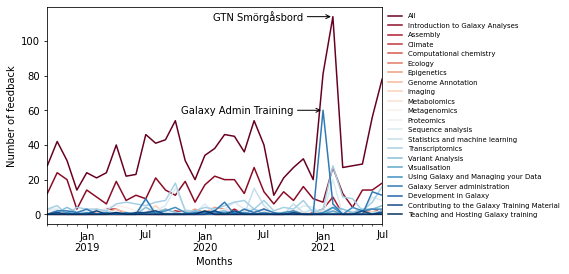
\includegraphics[width=0.45\textwidth]{images/feedback.png}
	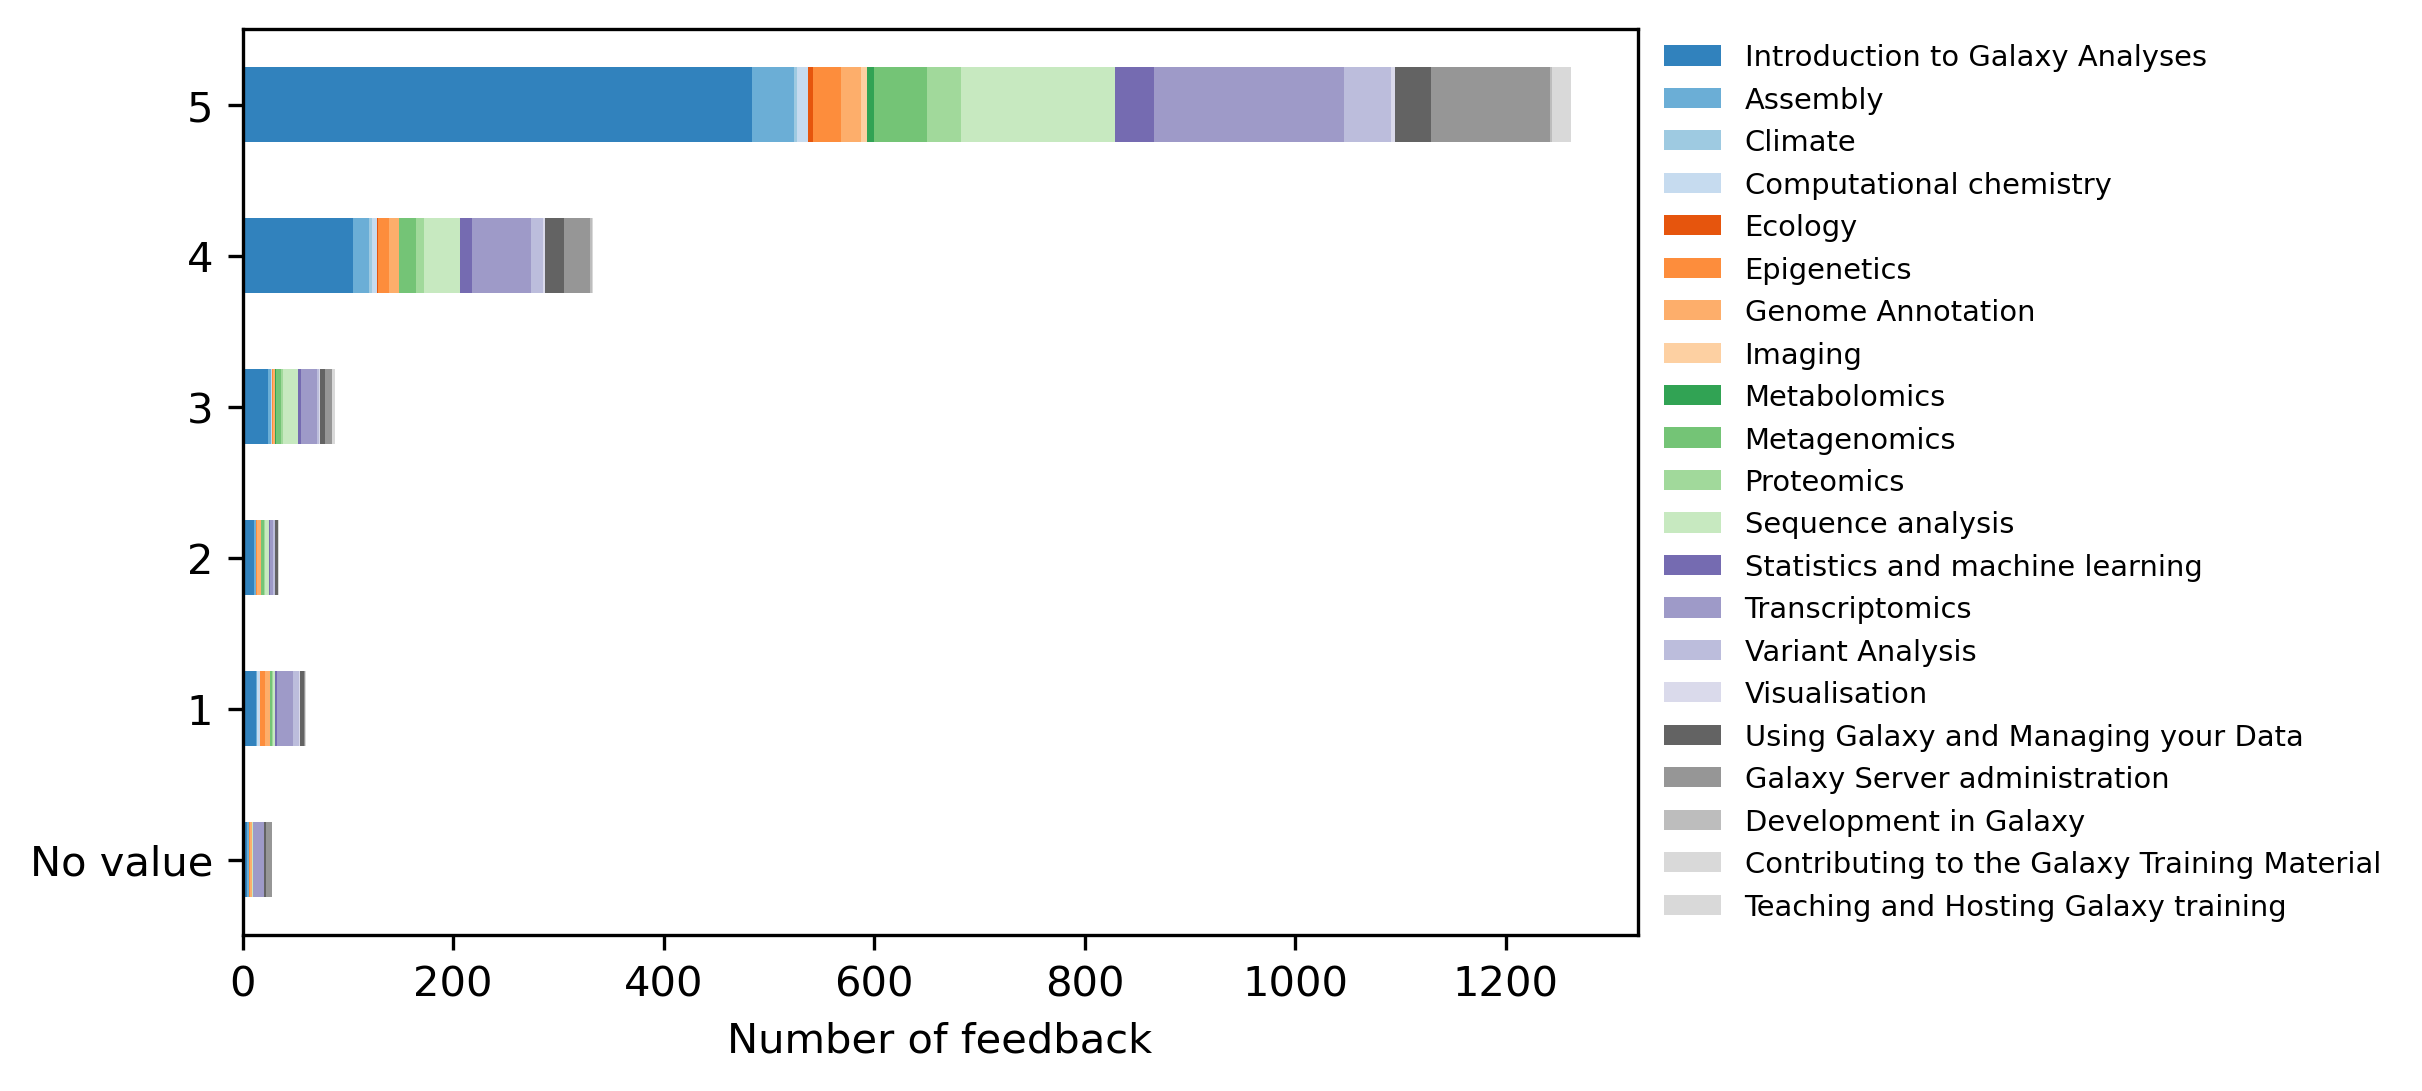
\includegraphics[width=0.45\textwidth]{images/feedback-scores.png}
	\caption{Number and results of the embedded feedback in the tutorials. 3 questions are asked in the form: ``How much did you like this tutorial?'' (from 1 to 5), ``What did you like?'', ``What could be improved?''.
    \label{fig:feedback}}
\end{figure}

The results of the 2020 trainers survey confirm these satisfaction scores. The participating instructors mostly gave 4 or 5 star ratings to the GTN tutorials, with 85.7\% of respondents indicating they would absolutely recommend them.
In addition to the training material, trainers sometimes use resources for enrollment forms and certifications, or add exercises.
Trainers report the need of a few weeks to prepare new material.
This time is reduced to a couple of days when the material already exists in the GTN\@.
They appreciate that the GTN material is “up-to-date”, stable, and that the community provides a wide variety of analysis relevant to current research.
The trainings are “easy to follow”, have a “great pedagogy” and allow trainees to be “involved in learning”.
The use of GTN material allows them to have more time to focus on the fundamental principles of  analyses and the specific needs of the trainees.
The surveyed trainers have been asked about the improvement they wished to see in the GTN resources.
One of the concerns is computational resources access, such as using public instances, or having backup servers if the server dedicated to the workshop encounters a problem.
Another important need is the access to GTN material metadata, like:  what new version of training has been published, what new training subject could require contributors.
Two-thirds of the surveyed trainers are contributors to the training material, and among those who are not, 90\% declare planning to become one in the future.
Users suggest that the pedagogic value of training materials could be improved by directing the users to different training depending on their level of expertise, and to provide more context to the analyses.
Some trainers would like more interactivity with the tutorials through exercises or through facilitating the parallel between the tutorial and the galaxy instance.


\subsection*{An Instructor's View: Teaching with Galaxy}

The GTN training materials minimize the amount of time and effort required for instructors to prepare for and run their course or workshop. Below we describe the process instructors go through for preparation and teaching of their course using GTN materials.


\subsubsection*{Preparing a course or workshop}

As an example, we take an instructor who plans to give a workshop on RNA-Seq data analysis to participants who never used Galaxy and never analyzed RNA-Seq data before.
In the category “Introduction to Galaxy Analyses” on \url{https://training.galaxyproject.org}, they find several HTML-based slides designed as a brief introduction to the Galaxy ecosystem and multiple hands-on tutorials -each with different stories- to introduce the basics of the Galaxy platform.
Each tutorial starts with a list of requirements, the expected level of learners, a rough time estimate, questions addressed by the tutorial, as well as learning objectives following the Bloom’s taxonomy \cite{TODO}.
These rich metadata components help the instructors to identify the best tutorial given their goals and audience.
By their hands-on nature, the tutorials rely on some predefined data and required tools.
To support instructors in their preparation, a link to the required datasets on an online repository hosted at CERN, Zenodo (\url{https://zenodo.org}), is provided on the top of the tutorial with also a list of Galaxy servers whose have the required tools and a workflow to test the tutorial.
The training material portfolio is also archived every month and available on Zenodo for local build to not risk last minute breakages.

\subsubsection*{Teaching the workshop}

During the workshop, following the tutorial script, the instructor shows in a step-by-step fashion with explanations (boxes) how to interact with Galaxy, upload data, run tools, extract workflows, etc and introduces the concepts of accessibility, reproducibility, and transparency. %% in the intro we mention (#274): "accessible, reproducible, and transparent computational research", hence we should probably write "accessibility, reproducibility and transparency" here.
Along the tutorials, question boxes with solutions are also available as self-assessment but also as help for instructors to interact with the participants. Other boxes are present to support the instructors, especially in their preparation.
For example, the detail boxes explain certain algorithmic aspects or compare different tools.
At the end of the tutorial, some take home messages are provided, but also link to possible follow-up tutorials.
Combined with the pre-requisites, they can be used to build a learning path or curriculum.
For example, for RNA-Seq data analysis, the instructor builds a curriculum with an introduction to Galaxy, followed by introduction to quality control, mapping and then RNA-seq data analysis.

\verb+gather feedback with form at end of tutorial+

\subsection*{User Stories}

The GTN materials are actively used by the community, in a wide range of settings and application domains [TODO: stats].
Below we describe a number user stories collected from instructors using the GTN tutorials.

\subsubsection*{(Post-)Graduate courses}

Galaxy is being used as an integral part of Bioinformatics programs in undergraduate (Clermont Auvergne University, Texas A\&M University, Avans Hogeschool) and postgraduate (Agrocampus Ouest, Rennes University, Brest University, Clermont Auvergne University, Station Biologique de Roscoff, Melbourne University) courses, as well as internal bioinformatics training sessions (Friedrich Miescher Institute, French Bioinformatics Institute, Erasmus MC).
For undergraduate courses, Galaxy is often used initially to teach the concept of pipelines and workflows.
Galaxy is convenient to explain data types and metadata, how data is structured, and connected to a tool.
Students learn the importance of the tool versions, as tools can change subtly and significantly over time, and will impact their analyses. Teachers can likewise showcase the evolution of algorithms over time using different versions of tools (e.g.\ bowtie and bowtie2) to help students understand the advances in the field. Galaxy can be used to show complete analytics workflows.
Without the need to spend resources on teaching basic Unix and command line skills, the time can be fully used to introduce each step (data cleaning, data analysis and visualization) and to go into details of each tool.
The postgraduate courses as the internal ones are, directed to biologists who are not comfortable working with the command line.
However, we often notice that beginners in bioinformatics like to initiate themselves with Galaxy as a step towards learning computer languages and working with the command line.
Here Galaxy can help to introduce the users to classical tools suites and approaches without diving into the command line and scheduling system environment.
Thus, it easily allows the course organisers to have both life scientists without any coding skills and users with knowledge in the same audience. The focus is on the tools, their parameters and the scientific meaning.
After getting familiar with each analysis step and understanding the meaning of parameters of each tool, it’s easier to go to command line environments to analyse high throughput data.


\subsubsection*{Training biomedical research scientists}
Biomedical science is a rapidly evolving field, and heavily reliant on bioinformatics

\subsubsection*{Citizen Science: Ecology}

\verb+TODO: Yvan+

\subsubsection*{Citizen Science: Beer Decoded}

To introduce biology and genomic sciences to the public and make pupils and citizens aware about DNA, sequencing technologies, bioinformatics, open science and their applications as well as their impact on their daily life, the street science community (\url{https://streetscience.community}) has been initiated.
Practical workshops are offered to identify microbes involved in brewing beers by the use of the Oxford Nanopore sequencing device MinION\@.
The participants learn to perform simple laboratory tasks and gain knowledge about microbes, DNA, sequencing and bioinformatics.
The European Galaxy server provides its own subdomain for the streetscience project (\url{https://streetscience.usegalaxy.eu}) with dedicated tools.
For the subsequent data analysis of the hundreds of microbes sequenced, a Galaxy workflow was created to identify their taxonomy.
Thanks to the graphical user interface, the participants can easily use the Galaxy framework to process the generated sequencing data from data upload to  metagenomics analysis.
Kraken2 \cite{wood2019improved} is a recommended metagenomics tool for Nanopore data and generates a report in a tree-like structure which can be downloaded or visualized further with Galaxy as an interactive pie chart.
Combining lab work and bioinformatics data analysis with Galaxy makes it very vivid to demonstrate the challenges and possibilities that genomics brings to our society.


\subsubsection*{Underrepresented Communities: Africa}


Reliable internet access is often taken for granted by researchers.
Bottlenecks in infrastructure may however cause significant issues for bioinformatics training as many students at once try to upload or download data.
This is especially problematic in low or middle income countries (LMICs) where internet access may be intermittent, restricted or completely unavailable.
Trainers are often brought in from afar meaning that the teaching takes places in a, for the trainer, unfamiliar setting and on a strict time schedule limited by the return trip(s) of those involved.
It is therefore important to avoid or minimise unforeseen delays caused by incompatibilities with local infrastructure, connectivity failures or unforeseen updates forcing new software to be downloaded or queries to remote servers to fail.
The eBioKit was developed based on these needs and is an assembly of open source or free for academic use software along with key databases for bioinformatics.
Various versions of the eBioKit has been used for over a decade by organisations such as EMBnet, H3Abionet, SANBio, and BECA/ILRI to train hundreds of researchers and bioinformatics trainers in LMICs (10.1371/journal.pcbi.1005616).
Galaxy has been a part of the eBioKit for most of its existence and was selected as key component for the eB3Kit which was developed in the B3Africa project \cite{Klingstrom_2016} to support biobank integrated research by combining the Baobab LIMS for biobanking (10.1089/bio.2017.0014) with software administration, data collection support and a Galaxy-based bioinformatics platform with a specialised workflow interface \cite{Klingstrom_2017}.
For training the Docker images provided by the Galaxy Training Network can easily be installed in a plug and play manner on the eBioKit or eB3Kit using Docker.
The selected material, installed beforehand, is then brought on a portable server to the training local and made available on the local network.
Students can then access it through the network and work directly on the server, which avoids installation issues for the students, unforeseen updates of web services, or other failures.


\subsubsection*{Remote and hybrid teaching: Australia \& Gallantries}

\verb+F2F training not always possible (e.g. COVID19), remote or hybrid format lowers socio-economic, geographical barriers+


\subsection*{A Contributor's View: developing GTN tutorials}

The GTN training materials repository is inherently collaborative and community-driven, and comprises a growing number of contributors with expertise in a wide range of scientific and technical domains. Given this highly collaborative nature of a community with very different skill sets, we continually strive to lower contribution barriers for content creators by providing a framework that is easy to use for training developers regardless of their level of knowledge of the underlying technical framework.

To this end, we aim to adhere to the best-practice guidelines described in  “Ten simple rules for collaborative lesson development” \cite{Devenyi_2018}.
Table~\ref{tbl:tensimplerules} describes these ten recommendations and their implementation within the GTN training material framework.

\begin{table}[]
	\centering
	\caption{Implementation of the ``Ten simple rules for collaborative lesson development''\cite{Devenyi_2018} in the training material
    \label{tbl:tensimplerules}}
	\begin{tabular}{p{0.5\textwidth}p{0.5\textwidth}}
		Rules & Implementation in the training material \\
		Clarify audience & Tutorial metadata includes level indicators (introductory, intermediate, advanced) and a list of prerequisite tutorials as recommended prior knowledge. This information is rendered at the top of each tutorial. \\
		Make lessons modular & Learning paths \\
		Teach best practice lesson development & In order to support the community of training developers, a ``Contributing'' topic was created containing 10 tutorials describing how to create new content. Furthermore, quarterly online collaboration fest(CoFests) are organized, where contributors can get direct support  \\
		Encourage and empower contributors & Involve them in reviews. Mentor them. Encourage them to become maintainers. Planemo \\
		Build community around lessons & CoFests and Community calls. Chat \\
		Publish periodically and recognize contributions & Author list on tutorials. Hall of fame. Citation at the end of the tutorial. Tweet about new or updated tutorials. List of new or updated tutorials in community newsletter. Soon: publication of tutorials via article \\
		Evaluate lessons at several scales & PR review, Trainee feedback, Instructor feedback, Workflow testing \\
		Reduce, re-use, recycle & Snippets. Share content between tutorials. Small modular tutorials linked with learning paths \\
		Link to other resources & Citations. Gallantries? \\
		You can't please everyone & but we can try (several different Galaxy introduction tutorials). Aim to clearly state what the tutorial does and does not cover, at the start.  \\
	\end{tabular}
\end{table}
%% Maybe more description on what Planemo has to do in the table ?

Galaxy training materials have evolved over the years to facilitate the contribution and maintenance of the tutorials.
The structure of the tutorials and repository has been made modular with unified syntax and use of snippets enabling easy access for authors to common tips and tricks new users might need to know.
This system allows for easy updating of all tutorials, if there is a change in tools or interface.

\subsubsection*{Contribution Flow}

The GTN framework ensures easy contribution and maintenance, through a diverse set of tools and standards.
This section describes the typical process a tutorial contributor will go through when developing a new tutorial.

\paragraph*{Contributing Tutorials.} To get acquainted with the tutorial development methodology, contributors can consult a set of dedicated tutorial in the \emph{contributing} topic. These tutorials provide a step-by-step guide to creating a tutorial in the GTN framework. These tutorials range from technical guides concerning the markdown and jekyll format, to pedagogical best practices. These tutorial help create a first example tutorial. After completing the tutorial, the instructor can move on to writing their own tutorial.

\paragraph*{Planemo Training Development Kit.} Tutorials are written in Markdown \cite{}, using the jekyll \cite{} framework.
To simplify the process, we have created a \emph{Tutorial Development Kit} within the Planemo tool \cite{TODO}, which allows contributors to generate a tutorial skeleton from a Galaxy workflow as a starting point for tutorial creation.
This skeleton contains the metadata section, auto-generated hands-on boxes for every tool, template question boxes, and instructions for the tutorial creators about how to proceed. From this skeleton, tutorial developers now add fill in the metadata, add the scientific background and story between the hands-on boxes, and add some formative assessment questions and answers.
This process greatly reduced the development time, and allows tutorial creators to focus on the scientific content of the tutorial, rather than the technical implementation details of the jekyll framework.

In order to further lower the contribution barrier, this planemo command has been encapsulated into a webservice (\url{https://ptdk.herokuapp.com/}) wherein training material authors can point to a public workflow on one of the UseGalaxy.* servers, and generate the tutorial skeleton automatically.
This removes the need for contributors to install the Planemo tool.
 We have found that this approach saves time for not only the contributors but also the reviewers as the training materials contributed using this method adhere well to the training material’s style guide.


\begin{figure}[!ht]
	\centering
	\includegraphics[width=0.8\textwidth]{images/tool-in-tutorial.png}
	\caption{An automatically generated hands-on box using the Planemo Training Development Kit. This box corresponds to the running of a single tool. All of the relevant parameters have been automatically extracted from the workflow definition file used to generate the skeleton. Where parameters are left to their default values, they are not listed in this box, but where they must be changed from their default values, detailed hands-on instructions are provided.\label{fig:planemo}}
\end{figure}


Furthermore, to avoid duplication of content, we have developed a set of modular tutorial components, called \emph{snippets}, which can easily be re-used across tutorials.
For example, common tasks in Galaxy such as starting a workflow or creating a new history, will be steps in the majority of tutorials. In order to avoid duplication, and making it easier to apply updates to these common steps when the Galaxy interface changes, we have modularized these sections.
These snippets can be included at any place in a tutorial with a single import instruction.
This again allows tutorial developers focus on the scientific topic at hand, rather than the Galaxy interface steps.


% Zenodo
The Training development kit also offers commands to generate the auxiliary tutorial files, such as the \verb+data_library.yaml+ file.
This file which describes the required input datasets. All datasets used in tutorials are stored on Zenodo and associated with a Digital Object Identifier (DOI) making them citable and discoverable.
This Zenodo DOI can be provided as a parameter to the Planemo Training Development Kit, to autogenerate the data library configuration file.
This files makes it easy to populate a \emph{Shared Data Library} on a Galaxy server using the ephermeris tool \cite{TODO}, which will greatly speed up the process of configuring a Galaxy server to support the tutorial.



\paragraph*{Local Preview and Testing.} During development, training creators will want to preview how their tutorial will look online.
To this end, we have provided simple functions to generate a local preview of the entire website with a single command. Whenever the tutorial files are updated, the preview will be regenerated as well.
In addition to visual inspection of the generated web pages, our framework offers a suite of testing tools, allowing contributors to check that their tutorial meets the guidelines.
These tests include checks of whether all required metadata is present and in the correct format, whether any links within the tutorial are valid, and whether files are correctly formatted.
This will help contributors and reviewers to quickly identify potential problems with a tutorial.


\paragraph*{Peer Review.} Once a contributor is happy with its tutorial, he/she can create a \emph{pull request} (PR) to the GTN GitHub repository where all tutorials are kept.  (\url{https://github.com/galaxyproject/training-material}).
The contribution will then undergo a peer-review process.
This process is open to any volunteers from the community; they will check the tutorial, both in terms of formatting and scientific content.
These reviewers can make suggestions for updates, and start a discussion with the tutorial contributor(s).
Typically there will be two or three reviewers for any given pull requests.
Based on this feedback the contributor(s) will update the tutorial, and this cycle of update and review will continue until both contributor(s) and reviewers are happy with the training materials.
In order to aid the reviewers, all available tests in our framework are automatically run on incoming pull requests, using the Travis Continuous Integration framework (\url{https://travis-ci.org/}). %% HRH: or just add the URL, https://travis-ci.org/
These tests aid in the identification of any errors in the tutorial, and prevent non-compliant tutorials from being merged.

Community is how the GTN survives and thrives: instead of having a central authority for approving new training content or changes, we delegate the reviewing process to topic maintainers.
For each topic within the training materials, the GTN has encouraged several prominent community members who are regular contributors to step up as topic maintainers, people who feel responsible for content in that domain and are empowered to review, approve, and merge content in that topic.
Topic maintainers are not the only group encouraged to review new pull requests and content, anyone from inside and outside of the community is welcome and encouraged to review new training materials.
While non-maintainers cannot merge changes, their review contributions are an important part of this project.
Reviews are the cornerstone of this project as shown by our very active reviewers in Figure~\ref{TODO}




\paragraph*{Tutorial maintenance and feedback.} Tutorials are dynamic entities; underlying analysis tools receive updates, new tools are developed, and the Galaxy interface itself changes regularly.
As a result, tutorials must undergo regular updates as well to reflect the state-of-the-art in the scientific domain, and correctly reflect the latest available version of the tools and the Galaxy interface.

Instructors preparing for their next workshop often check the tutorials as preparation, and in the process identify the places where the tutorial should be updated.
If the instructors feel comfortable making these changes themselves, they can open a pull request proposing the changes.
If not, they can create an \emph{issue} on GitHub to request the changes.

Furthermore, learner feedback is one of the most valuable resources to inform training improvements.
Anybody using the tutorials will find a feedback form at the end of it, where they can indicate any mistakes in the tutorial, or make suggestions for more general improvements.

Any feedback received is posted publicly on the GTN GitHub repository (unless the user indicated it should remain private), enabling the entire community to view and address the feedback.
This public feedback ensures a short feedback loop between content consumers and the tutorial authors, and keeps the authors accountable for their content, as seen in our user reviews (Figure~\ref{fig:feedback}).


Many of the updates to the GTN framework have come from suggestion by learners in workshops.
As an example, during one workshop a participant complained of the trouble copying lists of URLs or other code blocks easily; as a result we realised we could implement a copy button which would automatically copy the text on click, and even implemented the feature before the next day of the course.


This open strategy for content creation and updates is paying off.
Since the beginning of the project in the middle of 2016, over 1,000 pull requests have been created to add or update tutorials (Table~\ref{tbl:pullRequestReviewing}).

\begin{table}[]
\begin{adjustwidth}{-2.25in}{0in} % Comment out/remove adjustwidth environment if table fits in text column.
	\centering
	\caption{Statistics about Pull Request on GitHub repository.\label{tbl:pullRequestReviewing}}
	\begin{tabular}{l|p{0.2\textwidth}p{0.2\textwidth}p{0.2\textwidth}p{0.2\textwidth}}
									        & Number & Reviews and comments (mean number per PR) & Reviewers (mean number per PR) & Duration (mean per PR) \\\hline
		Pull Requests to add tutorial(s)    & 135    & 9.3                                       & 2.7                            & 26 days\\
		Pull Requests to update tutorial(s) & 683    & 3.4                                       & 1.7                            & 11 days\\
		Other Pull Requests                 & 386    & 2.5                                       & 1.5                            & 5 days\\
	\end{tabular}
\end{adjustwidth}
\end{table}


Thanks to a fast turnaround (on average, it takes \~20 days between the opening of a pull request and its merge), tutorials are regularly updated and iteratively improved over time, keeping up the standard of high-quality and state of the art.
Indeed, each tutorial undergoes (on average) a pull request every month to update it. Some highly used tutorials, like the “Reference-based RNA-seq” tutorial, got over 50 pull requests over the last 3 years, on average one every 3 weeks (Table …).


\paragraph*{Community Support.} If contributors encounter difficulties in any part of their contribution process, or simply want to discuss some aspects of their tutorials, they can seek help on the Gitter GTN channel. This channel is always active due to the large community covering many time zones.
Additionally, they may participate in our quarterly online contribution fests designed to support contributors and collaborate on tutorial updates and additions.

The Galaxy Training Network community has grown significantly since its inception.
Within two years after the start of the project, we had 77 members who wanted to be recognised as contributors to the training materials.
In the past two years, we have doubled again to 150 recognised contributors.
All of these contributors are publicly recognised in our \emph{“Hall of Fame”} (\url{https://training.galaxyproject.org/training-material/hall-of-fame/}).
Notably, these are the subset of contributors who wanted to be recognised, numerous others have contributed small fixes and one-off corrections where they did not choose to self-identify as one of the contributors.



\subsection*{Robust Training Infrastructure}

In the workshop setup process, identifying affordable and reliable infrastructure is one of the most difficult problems for trainers to solve followed by locating or developing training materials problems.
The problems share significant commonalities but require very different skills.
Training materials development requires good writing skills, depth of knowledge about the biological topic, and foresight to plan for student questions or potential errors.
Training infrastructure development requires good system administration skills, depth of knowledge about the environment (often Linux), and the foresight to plan for required capacity and scaling.
Here we present several different approaches which all work in concert to provide re-usable solutions to these problems for trainers, removing the need for them to either manage the system themselves, or convince their local sysadmin to quickly develop the necessary Galaxy knowledge.
The needs of training infrastructure are significantly different from normal Galaxy usage; a server used in training must process within 5-15 minutes or the course must stop.
The provided, small (sub-sampled) training datasets help to achieve this goal.
In normal usage users run workflows or ad hoc analyses, but can accept 30 minute delays in their jobs being processed.

\subsubsection*{Training Infrastructure as a Service (TIaaS)}
After hearing many trainers privately raise the issue of the difficulty in locating training infrastructure, locating servers that can handle the specific requirements of a course and were available as a managed service, Galaxy Europe developed Training Infrastructure as a Service (TIaaS) {cite-pending-tiaas-paper}.
Here they offer Galaxy as a service, sending training jobs to a special queue to run faster, thereby ensuring that by using their normal Galaxy service for which they are already responsible, the scaling costs of hosting multiple trainings are easily mitigated, and there is only one Galaxy service to manage.
Before the course a trainer requests space for a training event, providing information on the course size and content, and the administrators approve or deny the request.
If approved, VMs are launched and attached to the UseGalaxy.eu cluster, providing computation space for that specific course.
When the course begins, students self-register in the course using a keyword provided to them by the trainer.

TIaaS has been widely used (Figure~\ref{fig:tiaas-map}).

\begin{figure}[!ht]
	\centering
	\includegraphics[width=0.8\textwidth]{images/tiaas-map.png}
	\caption{Training Infrastructure as a Service has scaled well with administration time and cost, since June 2018 Galaxy Europe has hosted 66 trainings with over 2800 students with minimal overhead.\label{fig:tiaas-map}}
\end{figure}


During training events involving the developers of TIaaS, they noticed that trainer time and effort was dedicated to ensuring that all students had completed a given step, before they could move on in the tutorial.
A dashboard was added to the TIaaS service providing insight and visibility into class progress, now trainers could monitor the completion progress of students without moving around the classroom, and could move forward with training more efficiently (Figure~\ref{fig:tiaas}).


\begin{figure}[!ht]
	\centering
	\includegraphics[width=0.8\textwidth]{images/tiaas.png}
	\caption{The dashboard provides anonymised observability into class progress, trainers can see at a glance if everyone has completed the quality control steps, or if there are any errors that they should ask the students to raise with the class.\label{fig:tiaas}}
\end{figure}

TIaaS has provided an excellent solution to the training infrastructure problem; trainers can utilise a managed service for their courses having someone to call if something goes wrong, the centralisation of administration means less duplication and waste, and it has been shown to scale well with increasing course loads whilst not exerting undue pressure on administrators of existing Galaxy servers.

\subsubsection*{Scaling Training}
Touched upon in the discussion of TIaaS is the problem of scaling, but this problem occurs in two directions: how to scale the students, and how to scale the infrastructure.
Classroom sizes are usually limited by the number of interested participants in the locale, as well as by the availability of suitable venues.
Infrastructure is similarly limited, but with hidden requirements; running through a tutorial by yourself may execute quickly and look like everything will run smoothly, but some tools have non-obvious memory or cpu requirements that may balloon when giving a training for 30 or 100 students.
Both of these issues require planning and some creativity to solve.
TIaaS works to provide scalable infrastructure, the setup underlying the UseGalaxy.eu service allows for the addition of compute resources as needed.
While capacity is available from them, if training needs extend beyond what is possible on their infrastructure, there is the chance to build a cluster on compute resources that a trainer has available (e.g.\ in AWS) and attach these to the UseGalaxy.eu server, providing for essentially infinite scalability of training infrastructure, limited only by the training budget.

\subsubsection*{Training with the Internet}
Improved internet access also makes the TIaaS offering from Galaxy Europe an increasingly valuable tool for work in LMICs.
Bandwidth limitations and low reliability means that even if internet access has improved markedly it is often not sufficient for bioinformatics work.
Using a Galaxy server located in a region with high quality Internet bypasses these issues as demanding uploads and downloads are kept between the Galaxy server and the external data resources while the process is controlled from a remote location with more limited internet (\url{https://galaxyproject.eu/posts/2017/12/10/b3africa/}, \url{https://galaxyproject.eu/posts/2019/11/02/tomas-klingstroem-training-update/}).
Training researchers to train themselves using the Galaxy Training Network materials thereby means that following a basic training session researchers can continue their training through self-studies and also obtain help not only by their personal contacts but also by the wider Galaxy community.
When high quality internet access is not available, the GTN has produced Docker images.
Every topic has its own docker image available on Quay.io, allowing offline training, independent from public galaxy instances. A bare-bones galaxy base image is decorated with the necessary tools, workflows, tours and optional data-libraries to follow the tutorials.
Tools are installed based on the workflow files in the tutorials, guaranteeing that the galaxy container will contain the correct tools and dependencies.
The shared data libraries can be included in the docker image, or automatically downloaded at the container run, reducing image size.
This provides an ideal training environment where internet access is restricted but data is available, including many LMICs.

\subsubsection*{Workflow Testing}
While running through the training material prior to a course is always good practice for a trainer, sometimes there isn't time.
Automated workflow testing can provide some reassurances to trainers, letting them know that a given tutorial will certainly work on their selected server.
For example the developers of the tool tbl2asn, concerned about outdated results being produced and submitted to NCBI, include code in their tool to cause it to fail if the version is more than a few months old.
Here, workflow testing could help the community of trainers, developers, and tool users work in concert to ensure training materials are known to be working.
By developing workflows in parallel with training materials, the GTN have built the foundation for workflow testing. A project was started by the European Galaxy Team (\url{https://github.com/usegalaxy-eu/workflow-testing/}) to take these workflows, write test cases for them, and then run them every month against a few servers before recording the results.
In lieu of running the tutorial yourself, comparing every output to check if the results are still as expected, automated workflow testing can provide reassurances that everything is functional in advance of a big workshop.

\subsubsection*{Training Data Libraries}
A convenience built by the UseGalaxy.* initiative is a service which ensures that all of the datasets referenced in the GTN, are available across an array of Galaxy servers (\url{https://github.com/usegalaxy-eu/shared-data}).
While the service was initially constructed for the use of the UseGalaxy.* project, it is open for anyone to join, allowing their administrators to have all of the necessary datasets for training pre-loaded into their servers, without any administration overhead.
By having training data pre-loaded, this decreases the required network transfer for a training event, instead of 50 students downloading the same file, loading it into Galaxy 50 times, a single copy exists on that server and can be reused as often as needed without incurring additional storage costs.


\section*{Conclusion}
%% HRH: feel free to correct, improve, enlarge, or rewrite 
From the start of the Galaxy project, education has been an important part. Offering training as part of conferences or in the form of dedicated workshops has helped to grow and foster the worldwide Galaxy community and has brought (Biological) data analysis to a broad audience. Lot's of training material has been collected and made available on the Galaxy project website. In its original form, the collection lacked a proper structure, and most of those ad-hoc assembled materials became out-of-date soon after publication.
The Galaxy Training Network has created the Galaxy Training Platform. It is maintained in GitHub and has made it possible to coordinate and structure all those previous efforts in a sustainable way. It makes it easy to manage, adding new tutorials and/or updating existing ones. Thereby, it has become a valuable resource for both the trainee and the trainers.



% TABLES, todo: move.

\begin{table}[]
	\centering
	\caption{Top 10 tutorials in terms of filled embedded feedback form. Table extracted using \href{https://github.com/bebatut/galaxy-training-material-stats/blob/master/src/extract_repo_content_stats.ipynb}{Jupyter Notebook} on 2019-04-12\label{tbl:toptentutorials}}
	\begin{tabular}{p{0.8\textwidth}p{0.15\textwidth}}
		Tutorial                                                             & Number of responses \\\hline
		A short introduction to Galaxy (Introduction)                        & 174 \\
		Galaxy 101 (Introduction)                                            & 80 \\
		Quality Control (Sequence analysis)                                  & 73 \\
		Reference-based RNA-Seq data analysis (Transcriptomics)              & 56 \\
		From peaks to genes (Introduction)                                   & 44 \\
		Visualization of RNA-Seq results with Volcano Plot (Transcriptomics) & 20 \\
		Mapping (Sequence analysis)                                          & 19 \\
		NGS data logistics (Introduction)                                    & 19 \\
		16S Microbial Analysis with mothur (extended) (Metagenomics)         & 16 \\
		RNA-Seq reads to counts (Transcriptomics)                            & 14
	\end{tabular}
\end{table}



\begin{figure}[!ht]
	\centering
	\includegraphics[width=\textwidth]{images/visits-per-month.png}
	\caption{Number of visits per month on http://training.galaxyproject.org/ given the Google Analytics stats.\label{fig:visits}}
\end{figure}

\begin{figure}[!ht]
	\centering
	\includegraphics[width=0.8\textwidth]{images/tiaas.png}
	\caption{The dashboard provides anonymised observability into class progress, trainers can see at a glance if everyone has completed the quality control steps, or if there are any errors that they should ask the students to raise with the class.\label{fig:tiaas}}
\end{figure}

\begin{figure}[!ht]
	\centering
	\includegraphics[width=0.8\textwidth]{images/commits.png}
	\caption{Graph of contributions to the training materials repository\label{fig:contributions}}
\end{figure}

\begin{figure}[!ht]
	\centering
	\includegraphics[width=0.8\textwidth]{images/tool-in-tutorial.png}
	\caption{Here we show an automatically generated snippet box, all of the relevant parameters have been extracted from the workflow. Where parameters are left to their default values, they are not mentioned. Where they are changed, detained instructions about the precise parameters and their names are documented.\label{fig:planemo}}
\end{figure}

\section*{Supporting information}

% Include only the SI item label in the paragraph heading. Use the \nameref{label} command to cite SI items in the text.
\paragraph*{S1 Fig.}
\label{S1_Fig}
{\bf Bold the title sentence.} Add descriptive text after the title of the item (optional).

\paragraph*{S2 Fig.}
\label{S2_Fig}
{\bf Lorem ipsum.} Maecenas convallis mauris sit amet sem ultrices gravida. Etiam eget sapien nibh. Sed ac ipsum eget enim egestas ullamcorper nec euismod ligula. Curabitur fringilla pulvinar lectus consectetur pellentesque.

\paragraph*{S1 File.}
\label{S1_File}
{\bf Lorem ipsum.}  Maecenas convallis mauris sit amet sem ultrices gravida. Etiam eget sapien nibh. Sed ac ipsum eget enim egestas ullamcorper nec euismod ligula. Curabitur fringilla pulvinar lectus consectetur pellentesque.

\paragraph*{S1 Video.}
\label{S1_Video}
{\bf Lorem ipsum.}  Maecenas convallis mauris sit amet sem ultrices gravida. Etiam eget sapien nibh. Sed ac ipsum eget enim egestas ullamcorper nec euismod ligula. Curabitur fringilla pulvinar lectus consectetur pellentesque.

\paragraph*{S1 Appendix.}
\label{S1_Appendix}
{\bf Lorem ipsum.} Maecenas convallis mauris sit amet sem ultrices gravida. Etiam eget sapien nibh. Sed ac ipsum eget enim egestas ullamcorper nec euismod ligula. Curabitur fringilla pulvinar lectus consectetur pellentesque.

\paragraph*{S1 Table.}
\label{S1_Table}
\begin{table}[]
\begin{adjustwidth}{-2.25in}{0in} % Comment out/remove adjustwidth environment if table fits in text column.
	\centering
	\caption{Top 10 tutorials in terms of visited pages given the Google Analytics stats. Table extracted using \href{https://github.com/bebatut/galaxy-training-material-stats/blob/master/src/extract_repo_content_stats.ipynb}{Jupyter Notebook} on 2019-04-12.\label{tbl:topViewedTutorials}}
	\begin{tabular}{ll}
		Tutorial                                                             & Average number of visits per month \\\hline
		Reference-based RNA-Seq data analysis (Transcriptomics)              & 1763 \\
		16S Microbial Analysis with mothur (Metagenomics)                    & 1418 \\
		Visualization of RNA-Seq results with Volcano Plot (Transcriptomics) & 1299 \\
		Quality Control (Sequence analysis)                                  & 1170 \\
		Galaxy 101 (Introduction)                                            & 768 \\
		Mapping (Sequence analysis)                                          & 701 \\
		Visualization of RNA-Seq results with Heatmap (Transcriptomics)      & 686 \\
		Genome annotation                                                    & 585 \\
		RNA-Seq reads to counts (Transcriptomics)                            & 575 \\
		General tutorial (Metagenomics)                                      & 500 \\
	\end{tabular}
\end{adjustwidth}
\end{table}

\paragraph*{S2 Table.}
\label{S2_Table}
\begin{table}[]
\begin{adjustwidth}{-2.25in}{0in} % Comment out/remove adjustwidth environment if table fits in text column.
	\centering
	\caption{Top 10 tutorials by number of Pull Request on the GitHub repository. Table extracted using \href{https://github.com/bebatut/galaxy-training-material-stats/blob/master/src/extract_repo_content_stats.ipynb}{Jupyter Notebook} on 2019-04-12.\label{tbl:topEditedTutorials}}
	\begin{tabular}{l|lll}
		Tutorials                           & Creation   & Number of Pull Requests & Mean duration between PRs\\\hline
		Reference-based RNA-seq             & 2016-10-05 & 78                      & 16 days\\
		16S Microbial Analysis with mothur  & 2017-02-12 & 55                      & 18 days\\
		Mapping                             & 2016-10-04 & 50                      & 22 days\\
		Quality control                     & 2016-10-04 & 45                      & 27 days\\
		De novo transcriptomics             & 2017-02-19 & 45                      & 20 days\\
		From peaks to genes                 & 2017-05-24 & 44                      & 15 days\\
		DNA Methylation data analysis       & 2016-10-05 & 42                      & 22 days\\
		De novo RAD seq                     & 2017-02-14 & 42                      & 28 days\\
		Reference-based RAD-seq             & 2017-02-14 & 40                      & 31 days\\
		Calling variants in diploid systems & 2016-08-19 & 40                      & 28 days\\
	\end{tabular}
\end{adjustwidth}
\end{table}


\paragraph*{S3 Table.}
\label{S3_Table}
\begin{table}[]
\begin{adjustwidth}{-2.25in}{0in} % Comment out/remove adjustwidth environment if table fits in text column.
	\centering
	\caption{Statistics about Pull Request on GitHub repository.\label{tbl:pullRequestReviewing}}
	\begin{tabular}{l|p{0.2\textwidth}p{0.2\textwidth}p{0.2\textwidth}p{0.2\textwidth}}
									        & Number & Reviews and comments (mean number per PR) & Reviewers (mean number per PR) & Duration (mean per PR) \\\hline
		Pull Requests to add tutorial(s)    & 135    & 9.3                                       & 2.7                            & 26 days\\
		Pull Requests to update tutorial(s) & 683    & 3.4                                       & 1.7                            & 11 days\\
		Other Pull Requests                 & 386    & 2.5                                       & 1.5                            & 5 days\\
	\end{tabular}
\end{adjustwidth}
\end{table}



\begin{table}[]
\begin{adjustwidth}{-2.25in}{0in} % Comment out/remove adjustwidth environment if table fits in text column.
	\centering
	\caption{Numbers of tutorials, slides, hands-on tutorials and other material per topics. \label{tbl:numberOfMaterials}}
	\begin{tabular}{p{2in}|p{0.8in}llp{0.8in}lll}
		Topics                                       & Introduction slide decks & Tutorials & Slide decks & Hands-on tutorials & Workflows & Data on Zenodo & Data on data library\\\hline
		Introduction to Galaxy Analyses              & 1                        & 8         & 1           & 7                  & 3         & 7              & 3\\
		Assembly                                     & 0                        & 4         & 3           & 4                  & 4         & 4              & 4\\
		Computational chemistry                      & 0                        & 4         & 0           & 4                  & 3         & 4              & 0\\
		Ecology                                      & 0                        & 5         & 0           & 5                  & 4         & 4              & 4\\
		Epigenetics                                  & 2                        & 5         & 2           & 5                  & 5         & 5              & 4\\
		Genome Annotation                            & 1                        & 4         & 2           & 4                  & 2         & 4              & 4\\
		Imaging                                      & 0                        & 2         & 0           & 2                  & 2         & 2              & 2\\
		Metabolomics                                 & 1                        & 3         & 0           & 3                  & 3         & 3              & 2\\
		Metagenomics                                 & 1                        & 5         & 0           & 5                  & 5         & 5              & 4\\
		Proteomics                                   & 0                        & 14        & 0           & 14                 & 13        & 14             & 9\\
		Sequence analysis                            & 0                        & 2         & 2           & 2                  & 2         & 2              & 2\\
		Statistics and machine learning              & 0                        & 4         & 0           & 4                  & 4         & 4              & 4\\
		Transcriptomics                              & 1                        & 19        & 3           & 18                 & 16        & 18             & 13\\
		Variant Analysis                             & 1                        & 6         & 0           & 6                  & 4         & 6              & 6\\
		Data Manipulation                            &                          & 7         & 1           & 6                  &           & 6              & \\
		User Interface and Features                  &                          & 4         & 0           & 4                  & 1         & 4              & 1\\
		Development in Galaxy                        & 1                        & 13        & 12          & 4                  &           &                & \\
		Galaxy Server administration                 & 1                        & 31        & 24          & 16                 &           & 6              & \\
		Contributing to the Galaxy Training Material & 1                        & 10        & 2           & 9                  &           &                & \\
		Teaching and Hosting Galaxy training         & 0                        & 5         & 1           & 4                  &           &                & \\
	\end{tabular}
\end{adjustwidth}
\end{table}


\section*{Acknowledgments}
Cras egestas velit mauris, eu mollis turpis pellentesque sit amet. Interdum et malesuada fames ac ante ipsum primis in faucibus. Nam id pretium nisi. Sed ac quam id nisi malesuada congue. Sed interdum aliquet augue, at pellentesque quam rhoncus vitae.

%\nolinenumbers


% Either type in your references using
% \begin{thebibliography}{}
% \bibitem{}
% Text
% \end{thebibliography}
%
% or
%
% Compile your BiBTeX database using our plos2015.bst
% style file and paste the contents of your .bbl file
% here. See http://journals.plos.org/plosone/s/latex for
% step-by-step instructions.
%

\bibliography{references}

%\begin{thebibliography}{10}

%\bibitem{bib1}
%Conant GC, Wolfe KH.
%\newblock {{T}urning a hobby into a job: how duplicated genes find new
  %functions}.
%\newblock Nat Rev Genet. 2008 Dec;9(12):938--950.

%\bibitem{bib2}
%Ohno S.
%\newblock Evolution by gene duplication.
%\newblock London: George Alien \& Unwin Ltd. Berlin, Heidelberg and New York:
  %Springer-Verlag.; 1970.

%\bibitem{bib3}
%Magwire MM, Bayer F, Webster CL, Cao C, Jiggins FM.
%\newblock {{S}uccessive increases in the resistance of {D}rosophila to viral
  %infection through a transposon insertion followed by a {D}uplication}.
%\newblock PLoS Genet. 2011 Oct;7(10):e1002337.

%\end{thebibliography}



\end{document}

